\section{Global Mirror Control}
\label{sec:mdp}

We are investigating the use of Markov Decision Processes (MDPs) to
implement the high-level control of which mirror should be in what position.
MDPs represent a general approach to modeling optimization
problems~\cite{puterman} and have been applied to a diverse set of
application areas. Examples include: robotics~\cite{ab10},
economics~\cite{bs98}, % experiment design~\cite{White93},
medical decisions~\cite{ahsr10}, manufacturing~\cite{yyl04},
agriculture~\cite{Kristensen03},
real-time scheduling~\cite{gtsg08}
and wireless spectrum management~\cite{mgc16}.

Here, we adopt the definition of Glaubius et al~\cite{gtsg08}
of a (discrete-time) MDP as a 5-tuple
$(\mathcal{X}, \mathcal{A}, T, R, \gamma)$, with \emph{states}
$\chi \in \mathcal{X}$, \emph{actions} $a \in \mathcal{A}$,
and a transition system, $T$, which gives probability
$P_T (\chi' \mid \chi, a)$ of transitioning from state $\chi$ to
state $\chi'$ on action $a$.
The reward function $R(\chi, a, \chi') \in \mathbb R_{\ge 0}$ describes the
reward that accrues when transitioning from state $\chi$ to
state $\chi'$ via action $a$, under a discount factor, $\gamma$,
to ensure convergence of the long term reward.

For a catoptric surface with $N_m$ motors, each of which has $N_s$
steps, we define a state to be a vector of $N_m$ motor positions,
each of which has a value between 0 and $N_s$.  This is illustrated
for a single-mirror, 2-motor (pan and tilt) surface in Figure~\ref{fig:mdp2}.
The transitions represent single steps for the drive motors.
Self-loops (not shown) would represent no motion.  In the figure,
only one motor at a time is allowed to be in motion.  To support simultaneous
motion, diagonal transitions would be added to the transition system, $T$.
The figure generalizes to additional mirrors by adding two
additional dimensions per mirror.

\begin{figure}[ht]
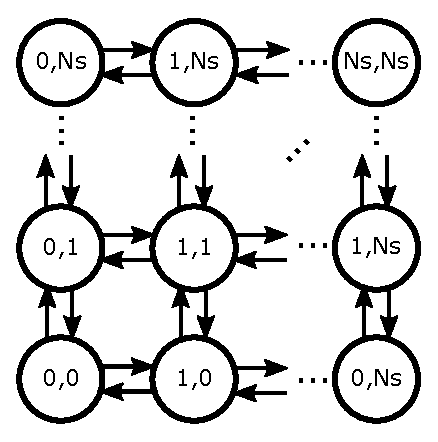
\includegraphics[width=0.5\columnwidth]{mdp2}
\caption{Single-mirror, 2-motor MDP state space and associated transitions.
Horizontal transitions represent moving the pan motor and vertical transitions
represent moving the tilt motor.}
\label{fig:mdp2}
\end{figure}

We define the reward function, $R$, as having multiple components. First,
it incorporates the match of the realized illumination pattern with a
desired illumination pattern. Second, it includes a measure of the impact
of mirror motion on the reliability of the mirror assemblies. Third, it
factors in the current positioning uncertainty due to running the
motors open loop (i.e., low undertainty when at the range limit, growing
uncertainty with each subsequent movement).

MDP theory~\cite{puterman} assures us that there exists a policy (choice
of action, $a$, in each state, $\chi$) that maximizes the expected reward.
While this policy is, in general, exponentially expensive
to compute, we are exploring heuristics that closely match the optimal
policy and are more computationally feasible in real time (so as to quickly
accomodate changes in sun position, desired illumination pattern, etc.).
